\part{The 3D graphics pipeline}
\frame{\partpage}

\begin{frame}{The 3D graphics pipeline}
	\begin{center}
		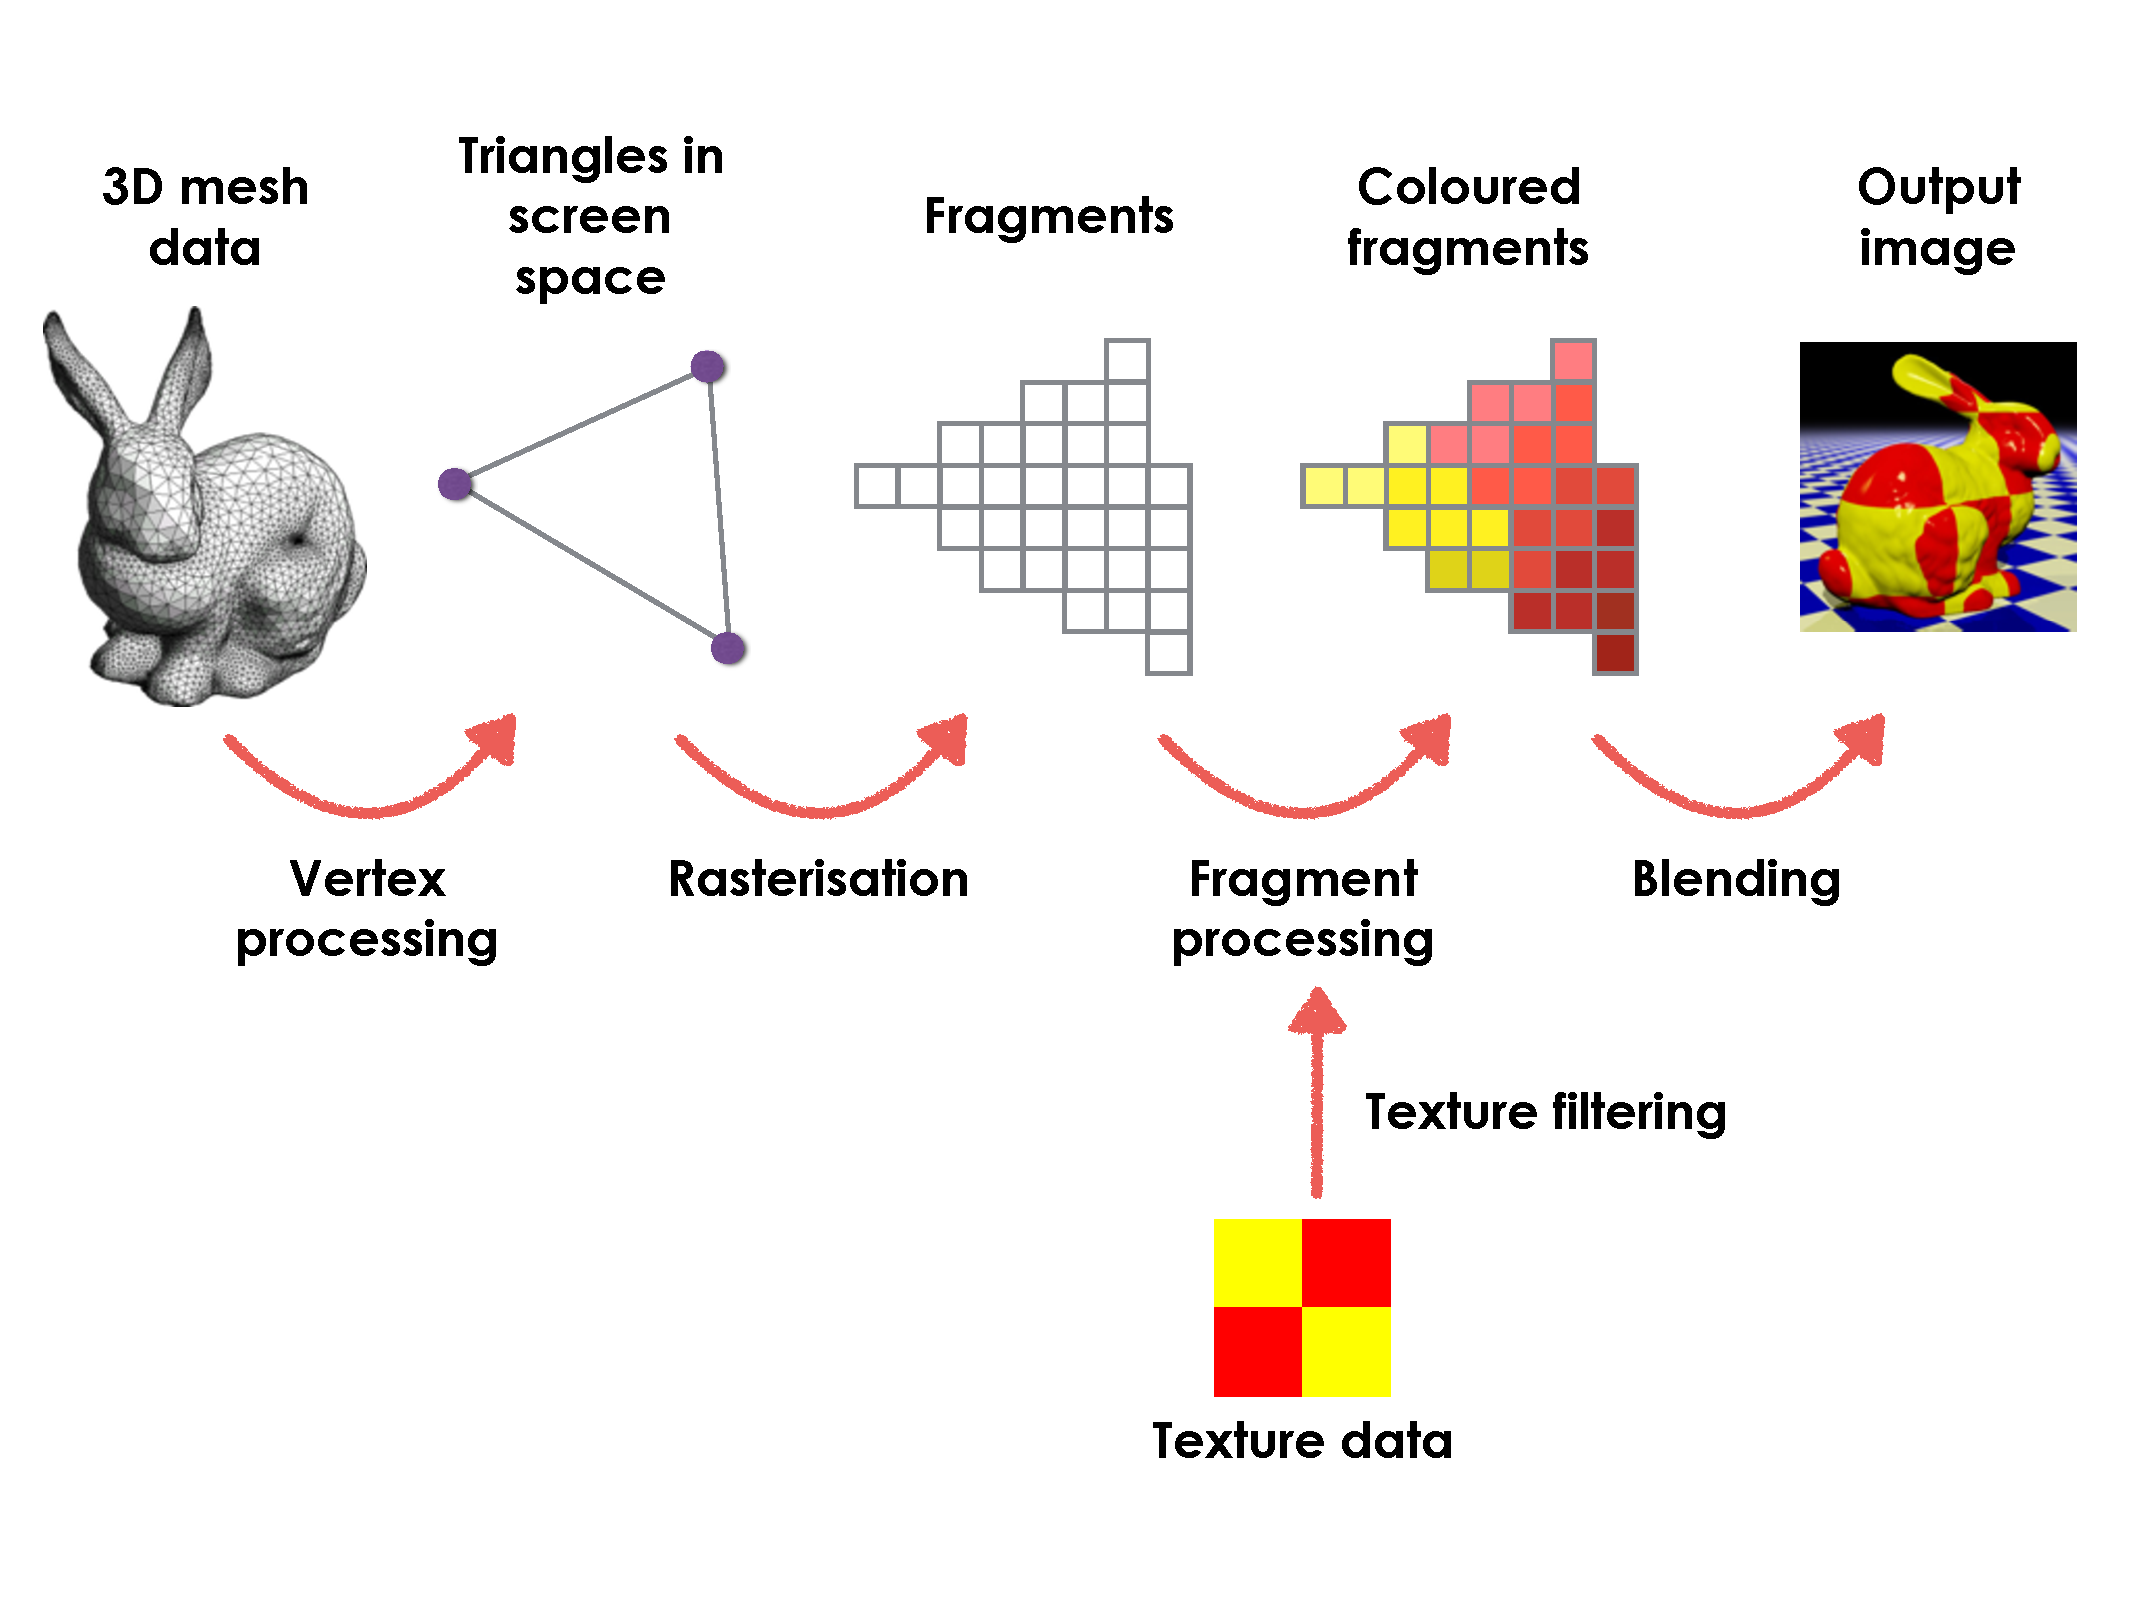
\includegraphics[height=0.7\textheight]{pipeline}
	\end{center}
\end{frame}

\begin{frame}{Vertex processing}
	\begin{columns}
		\begin{column}{0.3\textwidth}
			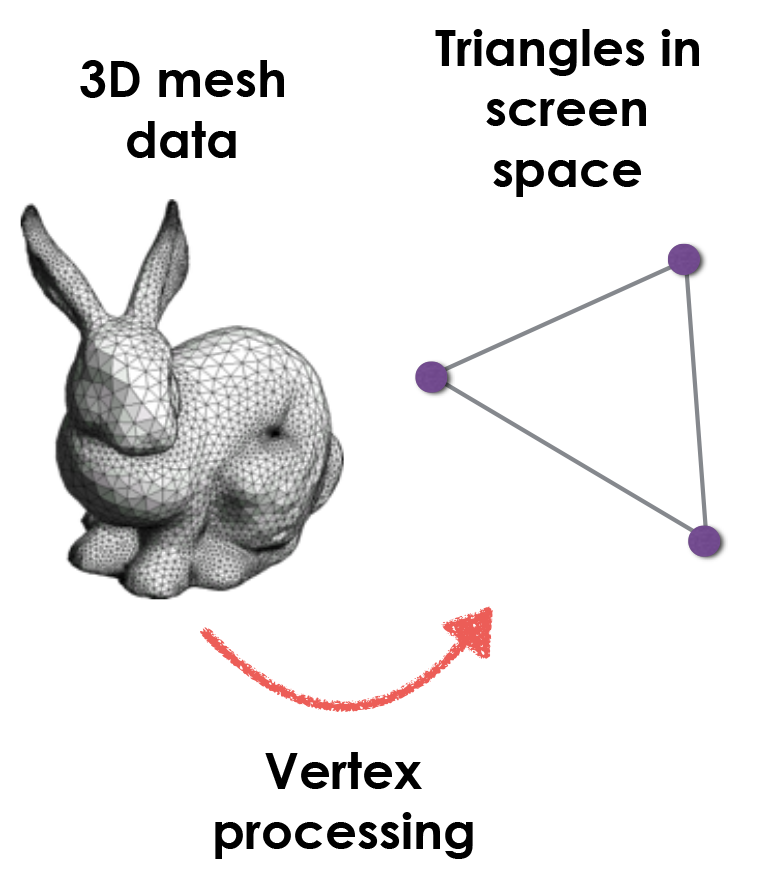
\includegraphics[width=\textwidth]{pipeline_1}
		\end{column}
		\begin{column}{0.65\textwidth}
			\begin{itemize}
				\pause\item Geometry is provided to the GPU as a \textbf{mesh} of \textbf{triangles}
				\pause\item Each triangle has three \textbf{vertices} specified in 3D space $(x,y,z)$
				\pause\item Vertex processor \textbf{transforms} (rotates, moves, scales) vertices
					and \textbf{projects} them into 2D screen space $(x,y)$
				\pause\item May also apply particle simulations, skeletal animations or deformations, etc.
			\end{itemize}
		\end{column}
	\end{columns}
\end{frame}

\begin{frame}{Rasterisation}
	\begin{columns}
		\begin{column}{0.3\textwidth}
			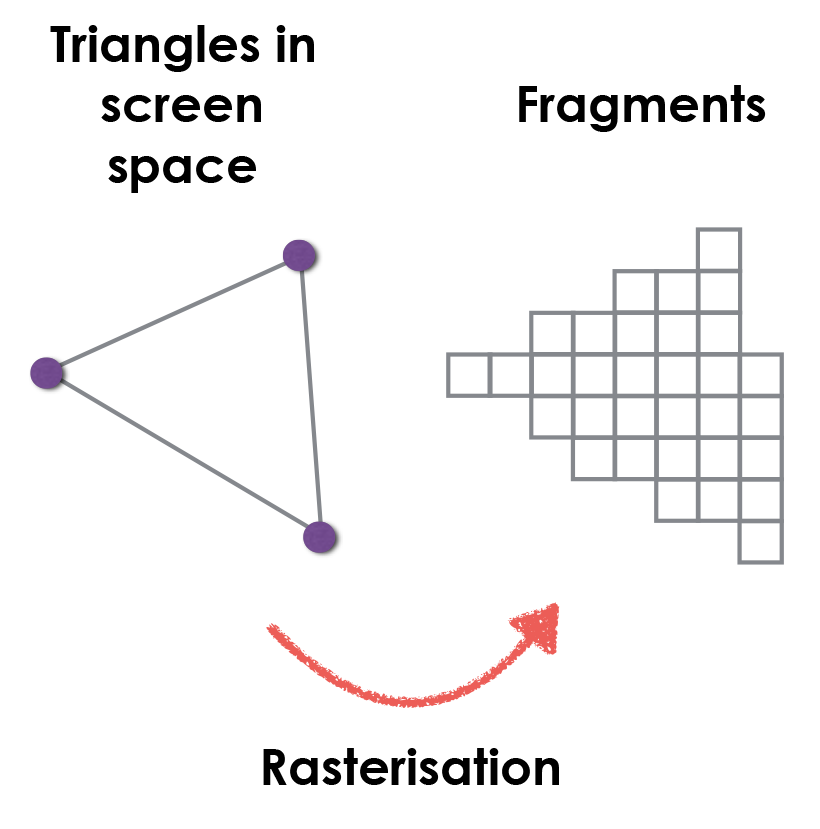
\includegraphics[width=\textwidth]{pipeline_2}
		\end{column}
		\begin{column}{0.65\textwidth}
			\begin{itemize}
				\pause\item Determine \textbf{which fragments} are covered by the triangle
				\pause\item In practical terms, ``fragment'' = ``pixel''
				\pause\item Vertex processor can associate \textbf{data} with each vertex;
					this is \textbf{interpolated} across the fragments
			\end{itemize}
		\end{column}
	\end{columns}
\end{frame}

\begin{frame}{Fragment processing}
	\begin{columns}
		\begin{column}{0.3\textwidth}
			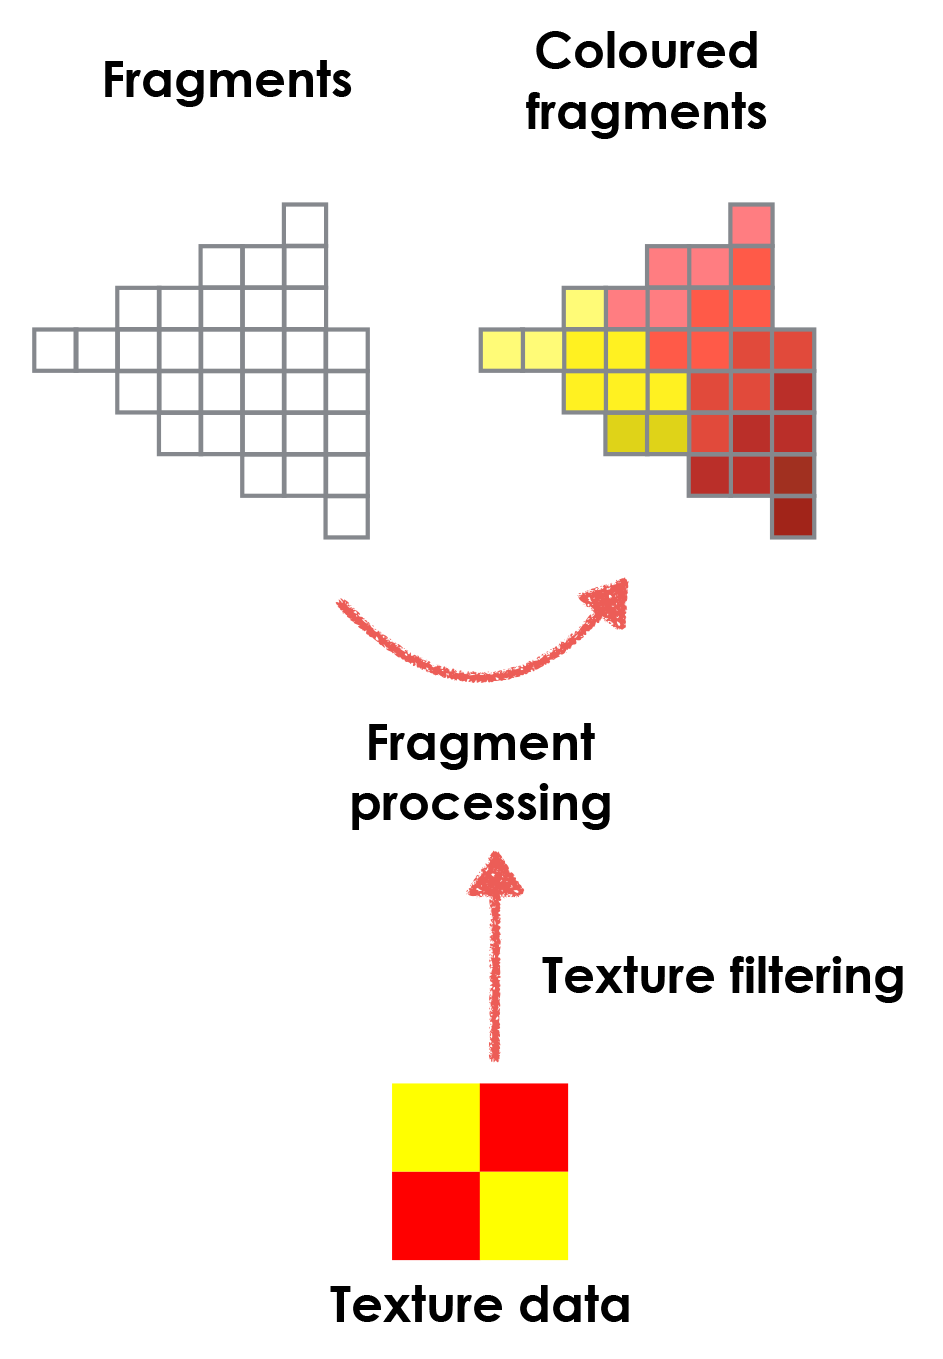
\includegraphics[width=\textwidth]{pipeline_3}
		\end{column}
		\begin{column}{0.65\textwidth}
			\begin{itemize}
				\pause\item Determine the \textbf{colour} of each fragment covered by the triangle
				\pause\item \textbf{Textures} are 2D images that can be \textbf{wrapped} onto a 3D object
				\pause\item Colour is calculated based on \textbf{texture}, \textbf{lighting} and other
					properties of the surface being rendered (e.g.\ shininess, roughness)
			\end{itemize}
		\end{column}
	\end{columns}
\end{frame}

\begin{frame}{Blending}
	\begin{columns}
		\begin{column}{0.3\textwidth}
			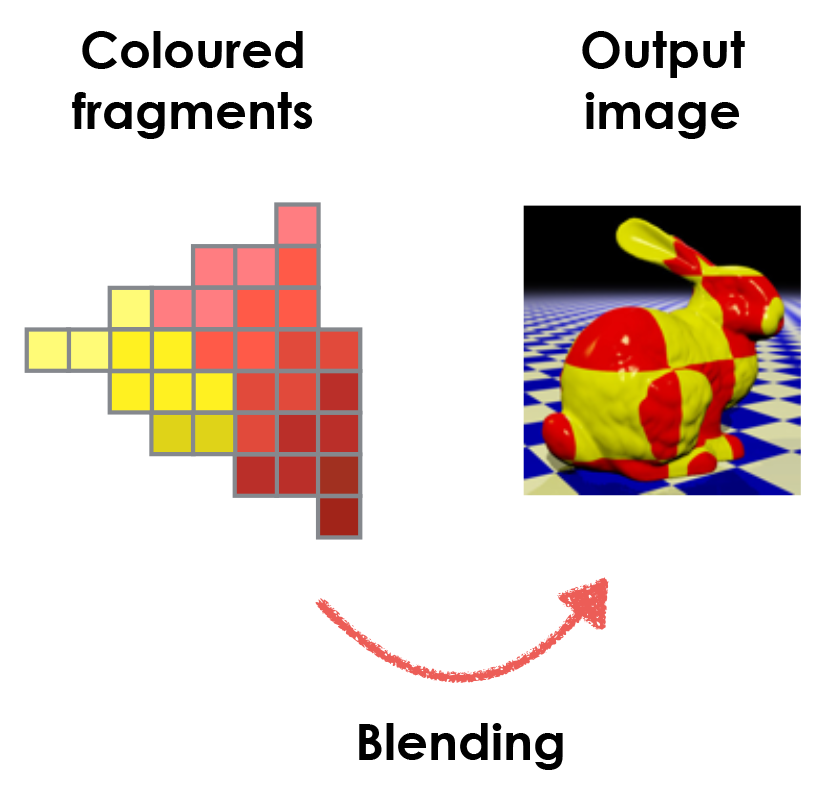
\includegraphics[width=\textwidth]{pipeline_4}
		\end{column}
		\begin{column}{0.65\textwidth}
			\begin{itemize}
				\pause\item Combine these fragments with the existing content of the image buffer
				\pause\item \textbf{Depth testing}: if the new fragment is ``in front'' of the old one, replace it;
					if it is ``behind'', discard it
				\pause\item \textbf{Alpha blending}: combine the old and new colours for a semi-transparent appearance
			\end{itemize}
		\end{column}
	\end{columns}
\end{frame}

\begin{frame}{Shaders}
	\begin{itemize}
		\pause\item The vertex processor and fragment processor are \textbf{programmable}
		\pause\item Programs for these units are called \textbf{shaders}
		\pause\item \textbf{Vertex shader}: responsible for geometric transformations, deformations, and projection
		\pause\item \textbf{Fragment shader}: responsible for the visual appearance of the surface
		\pause\item Vertex shader and fragment shader are separate programs,
			but the vertex shader can pass arbitrary values through to the fragment shader
	\end{itemize}
\end{frame}

